\chapter[Continuum Properties from $\mathcal{L}^2$ Functions]{Obtaining Continuum Properties from $\mathcal{L}^2$-Functions}


\section{Bound and Continuum States}
Before the decay of a metastable state is described one has to remember
that both bound and continuum states are involved in such a process.
Bound states are localized and in quantum mechanics
represented by square integrable
functions of the $\mathcal{L}^2$ Hilbert space. Their boundary conditions
lead to a quantized energy spectrum and the functions of the bound states
are normalized
to represent the $N$-particle wavefunction.
Unperturbed bound states are eigenstates of $H_0$ only
and can therefore conveniently be described using the time-independent
Schrödinger equation.
In contrast to the bound states the
continuum states are very delocalized, are not square-integrable
integrable and are hence not accessible for a probabilistic interpretation.
Their energy spectrum is continuous and the functions are normalized to
their respective energy.

In decay processes
where bound and continuum states interact, it is necessary to find a way to
properly represent bound states in an energy normalization or continuum states
in an $\mathcal{L}^2$ normalization.
Since most quantum chemical programme packages are based
on $\mathcal{L}^2$ functions,
it is most convenient to go for the latter approach.
Especially for properties like decay widths or ionization cross sections, one
possibility is to interprete the evaluation of an expectation value
including the continuuum in either the initial or the final state as
Gaussian quadrature and compare them to analogous expressions for the
expectation value in a discrete set of eigenstates. The given equivalence
allows to use the machinery of Gaussian quadrature combined with an imaging
procedure, both known in the literature,
for the determination of the required entity. \cite{Reinhardt79}

After an explanation of Gaussian quadrature it is going to be shown that
the discrete spectrum of a Hamiltonian in $\mathcal{L}^2$ representation
contains information of the continuum using Gaussian quadrature
based on the discussion of \cite{Reinhardt79}.
Then, it is going to be shown how the decay width can be obtained from a
discrete pseudo-spectrum by using Stieltjes imaging \cite{Langhoff76,Corcoran77}.
Finally we are going to introduce the FanoADC approach for the representation of
states in the $\mathcal{L}^2$ \ac{ISR} basis.



\section{Gaussian Quadrature}
The gaussian quadrature is a numerical method for integration.
The function to be integrated $g(x) = \rho(x) f(x)$ is approximated
to be a product of a positive definite weight
function $\rho (x)$ and a continuous and bounded function $f(x)$. \cite{Wikipedia_Gauss_Quadratur}
The evaluation of the integral is then obtained as

\begin{equation}
  \int\limits_a^b \rho(x) f(x) dx \approx \sum\limits_{i=1}^n \omega_i f(x_i)  .
\end{equation}

Here the weigths $\omega_i$ and the abscissae $x_i$ are to be determined
analytically, if possible, or otherwise in an optimal way. This leads the abscissae
to be unequally spaced unlike in the basic
integration schemes such as the trapezoidal rule.

The function $f(x)$ can be expressed as a polynomial.
For certain weight functions and boundaries
of integration, these
polynomials can be determined analytically.
It can furthermore be shown that the roots (zeros) of the highest order polynomial
describing the function $f(x)$ give the optimal abscissae $x_i$.
These polynomials $Q_n$ are normalized with respect to the weight function as

\begin{equation}
  \int\limits_{a}^{b} \rho(x) Q_n(x) Q_m(x) = N_n \delta_{nm}  ,
\end{equation}
where $N_n$ denotes the normalization factor.


In the special case of the weight function
$\omega(x)= \frac{1}{\sqrt{1-x^2}}$ and the interval $[-1,+1]$
the solution to the polynomials are the so-called Chebyshev polynomials, with
the analytical abscissae and weights

\begin{equation}
  x_{i,n} = \cos \left( \frac{2i-1}{2n} \pi \right)
  \quad\quad \omega_{i,n} = \frac \pi n 
\end{equation}

\begin{figure}[ht]
  \centering
  \begin{tikzpicture}
    \begin{axis}[%scale=0.8,
                 domain=-1.0:1.0,
                 samples = 200,
                 %xtick={-3.14159,-1.57089,...,3.14159},
                 %xticklabels={$-\pi$,$-\frac \pi 2$,0,$\frac \pi 2$,$\pi$},
                 cycle list name = exotic,
                 legend style={anchor= north west},
                 legend cell align = left
                 ]
     \addplot+[domain=-1:-0.965925826289+0.135517335117/2,
              diplom1,
              mark = none,
              %forget plot,
              pattern = north east lines,
              pattern color = diplom1
              ]
              {0.0987789349866} \closedcycle;
     \addlegendentry{approximation of the integral}
     \addplot+[domain=-0.965925826289+0.135517335117/2:-0.707106781187+0.370240244847/2,
              diplom1,
              mark = none,
              forget plot,
              pattern = north east lines,
              pattern color = diplom1
              ]
              {0.646446609407} \closedcycle;
     \addplot+[domain=-0.707106781187+0.370240244847/2:-0.258819045103+0.505757579964/2,
              diplom1,
              mark = none,
              forget plot,
              pattern = north east lines,
              pattern color = diplom1
              ]
              {0.982662411472} \closedcycle;
     \addplot+[domain=-0.258819045103+0.505757579964/2:0.258819045103+0.505757579964/2,
              diplom1,
              mark = none,
              forget plot,
              pattern = north east lines,
              pattern color = diplom1
              ]
              {1.017337588535} \closedcycle;
     \addplot+[domain=0.258819045103+0.505757579964/2:0.708718898022+0.370240244847/2,
              diplom1,
              mark = none,
              forget plot,
              pattern = north east lines,
              pattern color = diplom1
              ]
              {1.353553390592} \closedcycle;
     \addplot+[domain=0.708718898022+0.370240244847/2:1.0,
              diplom1,
              mark = none,
              forget plot,
              pattern = north east lines,
              pattern color = diplom1
              ]
              {1.901221065013} \closedcycle;
     \addplot [diplom2, thick]
              {x^3 + 1};
     \addlegendentry{$f(x)= x^3 + 1$}
     %\addplot [diplom3, thick]
     %         {x^4/4 + x};
     \addplot [only marks,mark=o,thick]
       coordinates {
                   ( 0.965925826289, 1.901221065013 )
                   ( 0.707106781187, 1.353553390592 )
                   ( 0.258819045103, 1.017337588535 )
                   (-0.258819045103, 0.982662411472 )
                   (-0.707106781187, 0.646446609407 )
                   (-0.965925826289, 0.0987789349866)
                   };
     \addlegendentry{$f_i(x_i)$}
    \end{axis}
\end{tikzpicture}

  \caption{Integration by Gauss-Chebyshev quadrature of the function
           $h(x)=x^3 + 1$ (dark blue) with $n=6$. The integral (light blue)
           is obtained by summation
           over all product of optimal abscissae and weights $x_ih(x_i)$ (circles).}
  \label{figure:gaussian_quadrature}
\end{figure}

This means, that the integration of an arbitrary function $h(x)$ within
the interval $[-1,1]$ can be integrated as

\begin{equation}
  \int\limits_{-1}^1 h(x) dx = \int\limits_{-1}^1 \omega(x) \sqrt{1-x^2} h(x) dx
  \approx \frac \pi n \sum\limits_{i_1}^n h(x_i) \sqrt{1-x_i^2}
\end{equation}

By appropriately transforming the variables, the limits of integration can be
chosen differently.

An example for such an integration is shown in Figure \ref{figure:gaussian_quadrature}
for $h(x) = x^3 + 1$. The dark blue curve shows $h(x)$, the points are the
calculated $h_i$ at the abscissae $x_i$ and the light blue hatched areas are the
approximations to the integral for the certain areas. Obviously, the finer the
grid for the integration, the more precise is the approximation to
the analytical integral.

The above discussion holds for a known weight function.
For an unknown weight function, the integral can be obtained by solving the so-called
moment problem. \cite{Reinhardt79}




\section{Expressing the Continuum Properties in Terms of Gaussian Quadrature}
Now the question arises how Gaussian quadrature can help to calculate
decay widths.
The Hamiltonian can be expressed in terms of a complete set of eigenfunctions

\begin{equation} \label{equation:complete_hamniltonian}
  H = \sum\limits_i \ket{\phi_i} E_i \bra{\phi_i}
     + \int\limits_0^\infty \mathrm{d}E \ket{\phi(E)} E \bra{\phi(E)}  ,
\end{equation}
where the manifold of $\phi_i$ denote the bound state eigenfunctions being orthonormal
in the sense of the probabilistic picture $\braket{\phi_j|\phi_i} = \delta_{ij}$.
The continuum functions $\phi(E)$ also form an orthonormal set of basis functions
but are normalized with respect to their energy.

\begin{equation}
  \braket{\phi(E) | \phi(E')} = \delta(E-E')
\end{equation}

In a calculation using a finite $\mathcal{L}^2$ basis, the diagonalization of the
Hamiltonian yields an approximative set of eigenfunctions $\chi_i$ with corresponding
eigenvalues $\tilde{E}_i$ such that

\begin{equation}
  \tilde{H} \ket{\chi_i} = \tilde{E}_i \ket{\chi_i} \quad\quad  \,
  \braket{\chi_j|\chi_i} = \delta_{ij} .
\end{equation}

The approximative Hamiltonian can be rewritten in terms of these $\mathcal{L}^2$
functions

\begin{equation} \label{equation:discrete_hamiltonian}
  \tilde{H} = \sum\limits_{E_i<0} \ket{\chi_i} \tilde{E}_i \bra{\chi_i}
            + \sum\limits_{E_j>0} \ket{\chi_j} \tilde{E}_j \bra{\chi_j}   ,
\end{equation}
where the first part with eigenvalues smaller than 0 corresponds to the
bound states and the second part with energies higher than 0 corresponds to
the continuum. In this representation the continuum is not described explicitly,
but in a discretized representation.

The eigenfunctions and eigenvalues of the positive energy solutions have no physical
meaning. Still, they inhibit a useful
mathematical meaning if the continuum part is interpreted in terms of
a numerical quadrature.
For this purpose the continuum part of the energy expectation value
$\braket{\Psi| H | \Psi}$ of the full Hamiltonian in
(\ref{equation:complete_hamniltonian}) is evaluated using Gaussian quadrature

\begin{align}
  \int\limits_0^\infty \mathrm{d}E \braket{\Psi|\phi(E)} E \braket{\phi(E)|\Psi}
  &\simeq \sum\limits_j \omega_j \braket{\Psi|\phi(E_j)} E_j \braket{\phi(E_j)|\Psi} ,
\end{align}
where  $\omega_j$ are the quadrature weights.
Compared to this the continuum part of the energy expectation
value of the discretized Hamiltonian $\braket{\Psi| \tilde{H} | \Psi}$ reads

\begin{equation}
  \int\limits_0^\infty \mathrm{d}E \braket{\Psi|\phi(E)} E \braket{\phi(E)|\Psi}
  \simeq \sum\limits_{E_j}  \braket{\Psi|\chi} \tilde{E}_j \braket{\chi|\Psi}   .
\end{equation}

In both cases, the integral is approximated by a sum and in some special cases,
where the analytic continuum functions are known, it can be shown from the results
that a one-to-one corespondence between each $\mathcal{L}^2$
eigenfunction of the positive energy part and the continuum function evaluated
at the energy $\tilde{E}_j$ exists. The so-called equivalent quadrature
weight $\omega_j^{Eq}$ connects the discrete and
the continuum function over a limited region of coordinate space
for the given energy and can be interpreted
as a renormalization \cite{Reinhardt79}.

\begin{equation}
  \ket{\chi_j} = \sqrt{\omega_j^{Eq}} \ket{\phi(\tilde{E}_j)}
\end{equation}

In the following, it is assumed that this equivalence between $\mathcal{L}^2$
and continuum functions with the integral interpreted as Gaussian quadrature
is valid for all systems under investigation.

Assumed for a moment the appropriate equivalent quadrature
weigths to be known, the decay width could ba calculated from a
discretized representation substituting the continuous basis
$\sum\limits_{r} \ket{\psi_r^{(-)}} \bra{\psi_r^{(-)}}$ of
equation (\ref{equation:Gamma_HE}) by the discrete basis
$\sum\limits_{r} \ket{\chi_r} \bra{\chi_r}$.

\begin{equation} \label{equation:gamma_moments}
  \Gamma = \frac 1{\omega_{j}^{Eq}} \left| \braket{\Phi_s|H-E|\chi_j} \right|^2
           \delta(E-E_j)
\end{equation}

Since in most cases, the weigth function is unknown, the weight function
is going to be calculated by solving the moment problem.
The following gedankenexperiment will show this possibility.
Consider the matrix element $\braket{\Phi_s|H\,H^k\,H|\Phi_s}$ is well defined.
Evaluating this matrix element for the Hamiltonian in the representation including
continuous functions as given in equation (\ref{equation:complete_hamniltonian})
yields

\begin{equation}    \label{equation:Gamma_mom_continuous}
 \braket{\Phi_s|H\,H^k\,H|\Phi_s} = \sum\limits_i \braket{\Phi_s|H|\phi_i}E_i^k
                                    \braket{\phi_i|H|\Phi_s}
   + \int\limits_0^\infty \mathrm{d}E \, \braket{\Phi_s|H|\phi(E)} E^k
     \braket{\phi(E)|H|\Phi_s}
\end{equation}

Substituting $H^k$ by $\tilde{H}^k$ of equation (\ref{equation:discrete_hamiltonian})
gives

\begin{equation}  \label{equation:Gamma_mom_discrete}
 \braket{\Phi_s|H\,\tilde{H}^k\,H|\Phi_s} =
   \sum\limits_i \braket{\Phi_s|H|\phi_i}\tilde{E}_i^k
     \braket{\phi_i|H|\Phi_s}
   + \sum\limits_j \braket{\Phi_s|H|\chi_j} \tilde{E}_j^k
     \braket{\chi_j|H|\Phi_s}
\end{equation}

The two seond terms approximately equal each other and additionally
they are the moments of the decay width, exact in equation
(\ref{equation:Gamma_mom_continuous})
and approximately in equation (\ref{equation:Gamma_mom_discrete}).

From the latter the moments are accessible as

\begin{equation}
  \Gamma^k = 2\pi \sum\limits_i E_i^k \left| \braket{\Phi_s|H-E|\chi_i} \right| ^2
           \delta(E-E_i)
\end{equation}
where orthogonality of $\Phi_s$ and $\chi_i$ is assumed. Otherwise the operators
in the equations would just need to be adjusted to $(H-E)$ in the formulation
of Fano or $H_{PQ}$ and $H_{QP}$ for Feshbach's formulation.



\subsection{Moment Problem}

The moments $S(k)$ of a real and continuous function $f(\omega)$ are defined
as \cite{MuellerPlathe90}

\begin{equation}
  S(k) = \int\limits_a^b \omega^k f(\omega) d\omega \quad\quad k=0,1,\dots  .
\end{equation}

In the case of $f(\omega)$ being a probability density function or a weight function
in the nomenclature of Gaussian quadrature, it is connected
to the probability distribution function $F(\omega)$ via
\begin{equation}
  F(\omega) = f(\omega){d\omega} .
\end{equation}

Note, that the standard assignment of variables in Gaussian quadrature and the
formulation of the moment problem is confusing. The equivalent weight function
and probability density is in Gaussian quadrature denoted by $\omega(x)$, while
in moment theory it is written as $f(\omega)$. We are going to stick to the
conventions of both fields.

The probability density function $f(\omega)$ is completely determined by the manifold
of moments. Therefore, when all moments are known, the probability density
function  (weight function) can be calculated from the moments.
In the present case $f(\omega)$
is the decay width $\Gamma(E)$, but the theory is also applicable and previously
used for the description of cross sections. Its pseudo-spectrum has the same
mathematical properties as the pseuso-spectrum of the decay width. Therefore,
the knowledge obtained in the description of cross sections can be adopted to
the description for the decay widths.

In practice, all moments are never available unless they can be
calculated analytically. Therefore, one has to approximately solve the reduced
moment problem since the density function is not completely defined.
In this case the $2r$ moments are

\begin{equation}
  S(k) = \int\limits_a^b \omega^k f(\omega) d\omega \quad\quad k=0,1,...,2r-1  
\end{equation}

In principle the moment problem can be solved by requiring the abscissae and
weights to reproduce a minimum number of moments. Unfortunately, this determination
is ill conditioned and, therfore one expresses the moments by orthogonal
polynomials of some known weight function. Then the
transformation to the polynomials is still ill conditioned, but the abscissae
and weights can be obtained by a well conditioned problem. \cite{Blumstein73}
The latter approach
of so-called modified moments has proved to be useful in the case of
properties such as the ionization
cross section and decay width.





\subsection{Finding the Gaussian Quadrature Abscissae and Weights from Modified Moments}

The procedure for the calculation of cross sections combining moment
theory and Gaussian quadrature has been investigated thoroughly. In this section
the argumentation of Müller-Plathe \cite{MuellerPlathe90} is followed, from which the
\verb|stieltjes| routine has been written by Averbukh and which is used in
combination with the FanoADC implemented in Dirac. The routine covers 
the construction of the polynomials, the calculation of abscissae and weights as well
as the Stieltjes Imaging. These topics are normally discussed together in the
literature \cite{MuellerPlathe89,Corcoran77,Langhoff76}.

For the ionization cross sections it has been shown that the moments with
$k>2$ diverge and hence are useless for the evaluation of the probability
density function $f(\omega)$. Therefore the inverse moments $S(-k)$ are investigated
instead:

\begin{equation}
  S(-k) = \int\limits_a^b \left( \frac{1}{\omega} \right) ^k f(\omega) d\omega
\end{equation}

For each \emph{order of Stieltjes} $r$, a set of
Chebyshev polynomials
$Q_n (1/\omega) = \sum\limits_{i=0}^n Q_n^{i}\left( \frac{1}{\omega} \right)^{i}$,
of order $0-r$ can be assigned, using $2r-1$ moments for their construction.
They are orthogonal with respect to the weight function
to be determined $f(\omega)$:

\begin{equation}
  \int\limits_a^b Q_n(1/\omega) \, Q_m(1/\omega) f(\omega) d\omega = N_n \delta_{nm}
\end{equation}

Chebyshev polynomials in general can be constructed from the recurrence formula
\begin{equation}
 Q_n(1/\omega) = \frac{1}{\omega - a_n} Q_{n-1}(1/\omega) - b_{n-1} Q_{n-2}(1/\omega),
\end{equation}

so that all polynomials can be constructed if $Q_0$ and $Q_1$ are known.
From these recursion relations, expressions for the recurrence coefficients
$a_n$ and $b_n$ can be obtained:

\begin{align}
  a_n     &= \frac{1}{b_0b_1\cdots b_{n-1}}
             \int (1/\omega)^n Q_{n-1}(1/\omega) f(\omega) d\omega
             - \sum\limits_{l=1}^{n-1} a_l  \label{equation:an_cont}\\
  b_{n-1} &= \frac{1}{b_0b_1\cdots b_{n-2}}
             \int (1/\omega)^{n-1} Q_{n-1}(1/\omega) f(\omega) d\omega \label{equation:bn_cont}
\end{align}

By expansion of the integral in equations \ref{equation:an_cont} and
\ref{equation:bn_cont} into a sum over moments obtained from the pseudo-spectra,
approximate expressions can be obtained for the recurrence coefficients
depending on the energies $\bar{\omega}_i$ (the inverse abscissae),
and couplings or the weights $\bar{f}_i$ of the
pseudo-spectrum.

\begin{align}
  a_n     &= \frac{1}{b_0b_1\cdots b_{n-1}}
             \sum\limits_{i=1}^N
               (1/\bar{\omega}_i)^n Q_{n-1}(1/\bar{\omega_i}) \bar{f}_i
             - \sum\limits_{l=1}^{n-1} a_l \label{equation:an_disc}\\
  b_{n-1} &= \frac{1}{b_0b_1\cdots b_{n-2}}
             \sum\limits_{i=1}^N
               (1/\bar{\omega}_i)^{n-1} Q_{n-1}(1/\bar{\omega}_i) \bar{f}_i
\end{align}

Hence, the recurrence relation now reads
\begin{equation}
  Q_n(1/\bar{\omega}_i) = \frac{1}{\bar{\omega}_i - a_n} Q_{n-1}(1/\bar{\omega}_i)
                          - b_{n-1} Q_{n-2}(1/\bar{\omega}_i)
\end{equation}

with
\begin{equation}
  Q_0(1/\bar{\omega}_i) = 1 \quad\quad Q_1(1/\bar{\omega}_i) = (1/\bar{\omega}_i) - a_1
\end{equation}
as starting points of the determination of the polynomials.

In order to determine the
distribution function $F(\omega)$ from the modified moments, the abscissae and
weights have to be calculated.
Again, the abscissae ($\omega_i$) are the roots of the
highest order polynomial
for each order of Stieltjes $r$

\begin{equation}
  Q_r(1/\omega_i) = 0 \quad\quad i = 1,2,\dots ,r .
\end{equation}

The connection between the weights and the polynomials is given by

\begin{equation}a  \label{equation:poly_weights}
  f_i = \left[ \sum\limits_{m=0}^{n-1} \frac{Q_m^2(1/\omega_i)}{N_m} \right]^{-1} .
\end{equation}

In order to obtain the roots of the highest order polynomial, in principle
any programm for root detection can be used. However, the problem can
be reformulated in terms of general polynomials $R_n(1/\omega)$ connected
to the obtained Chebyshev polynomials as
\begin{equation}
  Q_n(1/\omega) = (-1)^n \sqrt{N_n} R_n(1/\omega)
\end{equation}

with the respective recurrence formulas
\begin{equation}
  (1/\omega)R_{n-1}(1/\omega) = - \sqrt{b_n}R_n(1/\omega) + a_nR_{n-1}(1/\omega)
                                - \sqrt{b_{n-1}} R_{n-2}(1/\omega)
\end{equation}
and
\begin{equation}
  (1/\omega)R_0(1/\omega) = - \sqrt{b_1}R_1(1/\omega) + a_1 R_0(1/\omega) .
\end{equation}

Now, the roots can be determined from the following equation disregarding the
last vector as solution of the eigenvalue problem.

\begin{equation}
 \begin{split}
 \begin{pmatrix}
a_1        & -\sqrt{b_1}&            &                &             &          \\
-\sqrt{b_1}& a_2        & -\sqrt{b_2}&                &             &          \\
           & -\sqrt{b_2}& a_3        & -\sqrt{b_3}    &             &          \\
           &            & \ddots     & \ddots         & \ddots      &          \\
           &            &            & -\sqrt{b_{n-2}}& a_{n-1}     & -\sqrt{b_{n-1}}\\
           &            &            &                & -\sqrt{b_{n-1}}& a_n   
 \end{pmatrix}
 \begin{pmatrix}
  R_0(1/\omega)\\
  R_1(1/\omega)\\
  R_2(1/\omega)\\
  \vdots\\
  R_{n-2}(1/\omega)\\
  R_{n-1}(1/\omega)
 \end{pmatrix}         \\
 = (1/\omega)
 \begin{pmatrix}
  R_0(1/\omega)\\
  R_1(1/\omega)\\
  R_2(1/\omega)\\
  \vdots\\
  R_{n-2}(1/\omega)\\
  R_{n-1}(1/\omega)
 \end{pmatrix}
 -
 \begin{pmatrix}
  0\\
  0\\
  0\\
  \vdots\\
  0\\
  -\sqrt{b_n} R_{n}(1/\omega)
 \end{pmatrix}
 \end{split}
\end{equation}

Therefore the solution is simplified to diagonalization
of the coefficients matrix. Its eigenvalues are the roots of the polynomial
and hence the desired abscissae. The eigenfunctions $\mathbf{u_i}$ are normalized to 1.
For the determination of the weights $f_i$ from the eigenvectors
the following relation 

\begin{equation}
  1 = f_i \sum\limits_{m=0}^{n-1} R_m^2 (1/\omega_i) = \mathbf{u_i} \cdot \mathbf{u_i}
\end{equation}
of equation (\ref{equation:poly_weights}) has to be employed to give

\begin{equation}
  f_i = N_0 u_{0i}^2 
\end{equation}

Hence, the negative moments are approximated by the abscissae $(1/\omega_i)$ and
weights $f_i$ as
\begin{equation}
  S(-k) \approx \sum\limits_{i=1}^n (1/\omega_i)^k  f_i \quad\quad k=0,1,\dots,2r-1 
\end{equation}





\subsection{Stieltjes Imaging}
Having obtained the abscissae and weights, the probability distribution function
$F(\omega)$ can be approximated. For this purpose, the so-called Stieltjes imaging
is employed, where

\begin{equation}
  F^{(n)} (\omega) =
  \begin{cases}
    0                                & \omega < \omega_1\\
    \sum\limits_{j=1}^{i} f_j        & \omega_i < \omega < \omega_{i+1}\\
    \sum\limits_{j=1}^{n} f_j = S(0) & \omega_n < \omega 
  \end{cases}
\end{equation}
The procedure is illustrated in Figure \ref{figure:stieltjes_imaging} for a sixth
order Stieltjes imaging using a pseudo-spectrum for the NeAr ICD in a
Stieltjes histogram.


\begin{figure}[h]
  \centering
  %NeAr at 3.42 AA, 6th order of stieltjes
\begin{tikzpicture}
    \begin{axis}[%scale=0.8,
                 domain=-1.0:1.0,
                 samples = 200,
                 %xtick={-3.14159,-1.57089,...,3.14159},
                 %xticklabels={$-\pi$,$-\frac \pi 2$,0,$\frac \pi 2$,$\pi$},
                 cycle list name = exotic,
                 legend style={anchor= north west},
                 legend cell align = left,
                 xlabel= {$E$ [a.u.]},
                 ylabel= {$F(E)$}
                 ]
     \addplot+[domain=-1:-0.42789448546292908,
              diplom1,
              mark = none,
%              forget plot,
              pattern = north east lines,
              pattern color = diplom1
              ]
              {0.0} \closedcycle;
     \addlegendentry{$\sum\limits_{j=1}^{i} f_j \quad \omega_i < \omega < \omega_{i+1}$}
     \addlegendimage{empty legend}
     \addlegendentry{}
     \addplot+[domain=-0.42789448546292908:-0.25969072398345394,
              diplom1,
              mark = none,
              forget plot,
              pattern = north east lines,
              pattern color = diplom1
              ]
              {0.000790314507333} \closedcycle;
     \addplot+[domain=-0.25969072398345394:0.11385089684626037,
              diplom1,
              mark = none,
              forget plot,
              pattern = north east lines,
              pattern color = diplom1
              ]
              {0.00156501308103} \closedcycle;
     \addplot+[domain=0.11385089684626037:1.4305018410002852,
              diplom1,
              mark = none,
              forget plot,
              pattern = north east lines,
              pattern color = diplom1
              ]
              {0.00208878898366} \closedcycle;
     \addplot+[domain=1.4305018410002852:5.1882229137192883,
              diplom1,
              mark = none,
              forget plot,
              pattern = north east lines,
              pattern color = diplom1
              ]
              {0.0022929712885} \closedcycle;
     \addplot+[domain=5.1882229137192883:6,
              diplom1,
              mark = none,
              forget plot,
              pattern = north east lines,
              pattern color = diplom1
              ]
              {0.00241086375443} \closedcycle;
%     \addplot [diplom2, thick,
%               domain=-0.5:6]
%              %{0.001300 * ln(x+2.594992)};
%              {0.001049 * sqrt(x+1.374436)};
%     \addlegendentry{$F(x)= \frac 13 x^3 + x^2 + 2x$}
     \addplot [samples=200,mark=*,thick,smooth,diplom2]
       coordinates {
                   (-0.42789448546292908, 0.0003951572536665)
                   (-0.25969072398345394, 0.0011776637941815)
                   ( 0.11385089684626037, 0.001826901032345)
                   ( 1.4305018410002852, 0.00219088013608)
                   ( 5.1882229137192883, 0.002351917521465)
                   };
     \addlegendentry{$\approx F(E_i)$}
    \end{axis}
\end{tikzpicture}

  \caption{Stieltjes histogram of a sixth order integration from
           a NeAr ICD pseudo-spectrum (light blue). At the abscissae $\omega_i$,
           the histogram provides lower and upper bounds for the actual
           values. The mean of these two bounds (dark blue) is normally a good
           approximation of the distribution function $F(E)$ at this point.}
  \label{figure:stieltjes_imaging}
\end{figure}

This procedure is based on the so-called Chebyshev inequalities

\begin{equation} \label{equation:Chebyshev_inequalities}
  F^{(n)}(\omega_i - 0) \le F^{(n+1)}(\omega_i - 0) \le F(\omega_i)
  \le F^{(n+1)}(\omega_i + 0) \le F^{(n)}(\omega_i + 0).
\end{equation}

This means that the distribution functions obtained from the Chebyshev
polynomials approaching the abscissae $\omega_i$ from below and from above
give lower and upper bounds to the actual value of the distribution
function at this particular point $F(\omega_i)$. In fact, the mean of these
two values usually is a very good approximation to the exact value:

\begin{equation}
  F^{(n)} (\omega_i) = \frac 12 \left[ F^{(n)} (\omega_i - 0)
                       + F^{(n)} (\omega_i+0) \right]
\end{equation}

Since the integral was evaluated
which was the equaling quantity for both the Gaussian quadrature ansatz
in equation (\ref{equation:complete_hamniltonian}) and the discrete spectrum in equation
(\ref{equation:discrete_hamiltonian}), the distribution function obtained from the
discrete pseudo-spectrum is normalized correctly.
This distribution function is then numerically differenciated via

\begin{equation}
  f^{(n)} (\omega) =
  \begin{cases}
    \frac 12 \frac{f_1}{\omega_1}    & \omega < \omega_1\\
    \frac 12 \frac{f_{i+1} + f_i}{\omega_{i+1} - \omega_i}
                                     & \omega_i < \omega < \omega_{i+1}\\
    0                                & \omega_n < \omega
  \end{cases}
\end{equation}

to give  $r-1$ non-zero points of the desired
density function $f(\omega)$, which are
subsequently interpolated. In the routine of Averbukh, a 
monotonicity-preserving piecewise cubic Hermite spline interpolation
is used for this purpose. Afterwards, the interpolated density function is evaluated
for the energy of interest, which is the resonance energy $E_r$ in case of the
autoionization processes.

\subsection{Quality and Stability of the Results} \label{section:quality_stieltjes}
The abscissae of the polynomials constructed from different orders
of moments alternate as is schematically shown in
Figure \ref{figure:stieltjes_density}, where each colour of points corresponds
to one order. Therefore, in an ideal world, where all these points exactly lie
on the desired desity function, the combination of all abscissae
and weights for the interpolation is beneficial.

\begin{figure}[h]
  \centering
   \begin{tikzpicture}[
          scale=1.0,>=stealth,domain=0.5:8,samples=100,
          declare function={
          xshift = 0.7;
          yshift = 0.3;
          gamma(\x) = 1.5/(\x+xshift)^2  +yshift;
          noise(\x) = 1.5*exp(-1.0*(\x+xshift))*cos(10*(\x+xshift) r);
          calcgamma(\x) = gamma(\x) + noise(\x);
        }]
     \small
%  \draw[very thin,color=gray] (-0.1,-0.1) grid (4.9,4.9);
  \draw[->,thick] (-0.2,0) -- (5.2,0) node[right] {$E$};
  \draw[->,thick] (0,-0.2) -- (0,4.2) node[above] {$\Gamma(E)$};
  % add ticks
  \draw [thick] (4,0) -- (4,-2pt) node [anchor=north] {$E_r$};
  \draw [color=black,domain=0:5,smooth,very thick]    plot
         (\x,{gamma(\x)}) node [anchor=south east] {density function};
  \foreach \x in {0.2,0.8,...,5}
    \fill[color=orange!80] (\x,{gamma(\x)}) circle (0.08);
  \foreach \x in {0.4,1.0,...,5}
    \fill[color=diplom1!80] (\x,{gamma(\x)}) circle (0.08);
  \foreach \x in {0.6,1.2,...,5}
    \fill[color=diplom2!80] (\x,{gamma(\x)}) circle (0.08);
%  \draw [color=red,domain=0.0:5,smooth,thick]    plot
%         (\x,{calcgamma(\x)}) node [above left=20pt] {real life};
 \end{tikzpicture}
 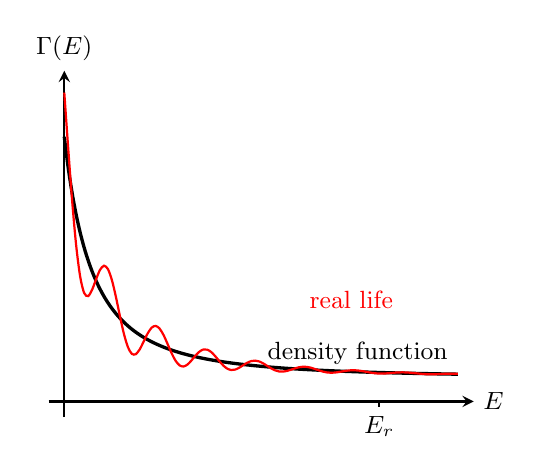
\begin{tikzpicture}[
          scale=1.0,>=stealth,domain=0.5:8,samples=100,
          declare function={
          xshift = 0.7;
          yshift = 0.3;
          gamma(\x) = 1.5/(\x+xshift)^2  +yshift;
          noise(\x) = 1.5*exp(-1.0*(\x+xshift))*cos(10*(\x+xshift) r);
          calcgamma(\x) = gamma(\x) + noise(\x);
        }]
     \small
%  \draw[very thin,color=gray] (-0.1,-0.1) grid (4.9,4.9);
  \draw[->,thick] (-0.2,0) -- (5.2,0) node[right] {$E$};
  \draw[->,thick] (0,-0.2) -- (0,4.2) node[above] {$\Gamma(E)$};
  % add ticks
  \draw [thick] (4,0) -- (4,-2pt) node [anchor=north] {$E_r$};
  \draw [color=black,domain=0:5,smooth,very thick]    plot
         (\x,{gamma(\x)}) node [anchor=south east] {density function};
%  \foreach \x in {0.2,0.8,...,5}
%    \fill[color=orange!80] (\x,{gamma(\x)}) circle (0.08);
%  \foreach \x in {0.4,1.0,...,5}
%    \fill[color=diplom1!80] (\x,{gamma(\x)}) circle (0.08);
%  \foreach \x in {0.6,1.2,...,5}
%    \fill[color=diplom2!80] (\x,{gamma(\x)}) circle (0.08);
  \draw [color=red,domain=0.0:5,smooth,thick]    plot
         (\x,{calcgamma(\x)}) node [above left=20pt] {real life};
 \end{tikzpicture}

  \caption{Schematic illustration of the interpolation after the
           stieltjes calculations to yield the density function $\Gamma(E)$,
           which is to be evaluated at the resonance energy $E_r$.
           Suppose the black curve to be the
           exact result. Then (left panel), for each order of Stieltjes calculation
           the points lie on this curve, where points from different orders
           (different colours of the points) intersect each other. The interpolation
           gives the exact result. In reality (right panel) the
           interpolations (even of one order of Stieltjes)
           are likely to show oscillations due to non-orthogonalities of
           Chebyshev polynomials in the higher orders and inaccurate descriptions
           due to a large gap between the lower and upper bounds for low
           orders.}
  \label{figure:stieltjes_density}
\end{figure}

As can be seen from the Chebyshev inequalities in
equation \ref{equation:Chebyshev_inequalities}, the higher the highest
power of the polynomials and hence the larger the degrees of freedom,
the closer the lower and upper bounds get to the exact result.

Unfortunately, the moment problem is ill-conditioned and by introducing
the polynomials, the moment problem as such get well-conditioned but instead
the construction of the polynomials from the pseudo-spectrum is ill-conditioned.
As can be seen from the Chebyshev inequalities, one would like to go to as
high orders as possible in order to get more accurate results. But in the construction
of the recurrence coefficients \ref{equation:an_disc}, two very large numbers
are subtracted from each other. This is known to be numerically unstable.
And the higher the order of the moment, the bigger
are these numbers and hence the introduced error. Therefore the number
of moments to be successfully employed for the approximation of the
density function is limited by the quality of the orthogonality of
the corresponding set of constructed polynomials. In the final density function
non-orthogonalities as well as errors from inaccurate descriptions of lower
orders can be detected by the presence of oscillations as shown in
Figure \ref{figure:stieltjes_density} in the right panel. In the case of the density
function being well behaved in the area of the resonance energy $E_r$, the
description might still be feasible. In case of strong oscillations, the validity
of the results is highly questionable. The interpolation can be smoothed
by taking only stable orders of stieltjes into account or, in other words,
by reducing the threshold of allowed non-orthogonality.

Another error is introduced by treating effects such as channel openings, which
are charaterized by discontinuities, with Gaussian quadrature which is valid
for smooth density functions only. 
